\documentclass{article}

% Document extensibility %
%
% Disables native paragraph indentation
\usepackage{parskip} 
%
% Provides further bullet options for lists
\usepackage{enumitem}

% Mathematical symbol and statement packages %
%
% Necessary
\usepackage{amsmath}
\usepackage{amssymb}
%
% Extensive fraction notation
\usepackage{xfrac}
%
% Generic mathematical commands
% Notable: \degree, \celcius
\usepackage{gensymb}
%
% Variable vector notation (arrow above variable)
\usepackage{esvect}
%
% Multiline boxed equations
\usepackage{empheq}
%
% SI Unit
\usepackage{siunitx}
\DeclareSIUnit\rev{rev}
\DeclareSIUnit\feet{ft}
\DeclareSIUnit\pound{lb}
\usepackage{physunits}
%
% More intuitive arrays/matrices
\usepackage{array}
%
% Linear Equations
\usepackage{systeme}
%
% Boxes!
\usepackage{mdframed}
%
% Matrix Notation
\usepackage{bm}

% Graphic packages %
%
% Diagrams and illustrations
\usepackage{tikz}
\usetikzlibrary{positioning}
%
% Image insertion
\usepackage{graphicx}

% LaTeX Commands
%
% Argument Parser
\usepackage{xparse}

% Document content %
%
% Change title of table of contents
% \renewcommand{\contentsname}{Title}

\title{Homework 9 - Circular Motion}
\author{Corey Mostero - 2566652}
\date{30 May 2023}

\begin{document}

% Command `\hr` to insert horizontal rules
\newcommand{\hr}{\par\noindent\rule{\textwidth}{0.4pt}}

% Command to box and center math equations
\newcommand{\bc}[1]{
	\begin{equation*}
		\begin{boxed}
			{#1}
		\end{boxed}
	\end{equation*}
}

% Command for single line equations with a condition
\newcommand{\cond}[2]{
	\ifmmode
		{#1} \quad {#2}
	\else
		$$ {#1} \quad {#2} $$
	\fi
}

% Matrix and Vector notation
\newcommand{\matr}[1]{
	\ifmmode \bm{#1}
	\else \textit{\textbf{#1}}
	\fi
}
\newcommand{\vect}[1]{
	\ifmmode \mathbf{#1}
	\else \textbf{#1}
	\fi
}

% Laplace
\NewDocumentCommand{\lap}{o}{
	\IfNoValueTF{#1}
		{ \mathcal{L} }
		{ \mathcal{L} \left\{ {#1} \right\} }
}
\NewDocumentCommand{\ilap}{o}{
	\IfNoValueTF{#1}
		{ \mathcal{L}^{-1} }
		{ \mathcal{L}^{-1} \left\{ {#1} \right\} }
}

\maketitle
\newpage

\tableofcontents

\section{Book}

\subsection{5.43}

\begin{align*}
	m & = \SI{0.80}{\kilogram} \\
	L & = \SI{0.90}{\meter} \\
	T & = \SI{60.0}{\newton}
\end{align*}
\begin{enumerate}[label = \textbf{(\alph*)}]
	\item Draw a free-body diagram of the stone.
		\begin{center}
			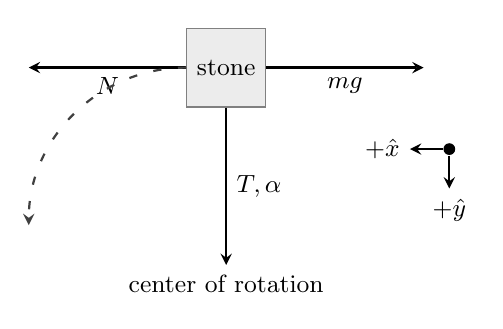
\begin{tikzpicture} [font = \small]
				\node at (0, 0) (origin) { center of rotation };
				\node [rectangle, draw = gray, fill = gray!15, minimum size = 1cm, above = 2cm of origin] (stone) { stone };
				\draw [thick, -stealth] (stone.south) -- (origin) node [midway, right] {$ T, \alpha $};
				\draw [thick, -stealth] (stone.west) -- ++ (-2cm, 0) node [midway, below] {$ N $};
				\draw [thick, -stealth] (stone.east) -- ++ (2cm, 0) node [midway, below] {$ mg $};
				\draw [thick, -stealth, black!75, loosely dashed] (stone.west) arc(90:180:2);

				\node [circle, fill, inner sep = 1.5pt, above right = 2cm of origin] (axis_point) {};
				\draw [thick, -stealth] (axis_point) -- ++ (0, -0.5cm) node [below] {$ +\hat{y} $};
				\draw [thick, -stealth] (axis_point) -- ++ (-0.5cm, 0) node [left] {$ +\hat{x} $};
			\end{tikzpicture}
		\end{center}
	\item Find the maximum speed the stone can attain without the string breaking.
		\begin{align*}
			\sum F_c & = m\alpha \\
			T & = m \left( \frac{ v_{max}^2 }{ L } \right) \\
			v_{max} & = \sqrt{ \frac{ TL }{ m } } \\
			v_{max} & = \sqrt{ \frac{ (\SI{60.0}{\newton})(\SI{0.90}{\meter}) }{ \SI{0.80}{\kilogram} } } \\
			v_{max} & = \SI{8.22}{\meter \per \second}
		\end{align*}
		\bc{ v_{max} = \SI{8.22}{\meter \per \second} }
\end{enumerate}

\subsection{5.45}

\begin{align*}
	m & = \SI{1.60}{\kilogram} \\
	v & = \SI{12.0}{\meter \per \second} \\
	r & = \SI{5.00}{\meter}
\end{align*}
\begin{enumerate}[label = \textbf{(\alph*)}]
	\item What is the normal force at point $ A $?
		\begin{center}
			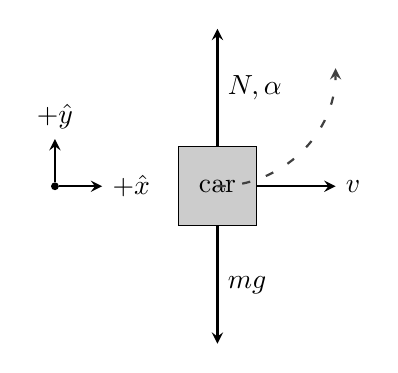
\begin{tikzpicture}
				\node [rectangle, draw = black, fill = black!20, minimum size = 1cm] (origin) { car };
				\draw [thick, -stealth] (origin.east) -- (1.5cm, 0) node [right] {$ v $};
				\draw [thick, -stealth] (origin.south) -- (0, -2cm) node [midway, right] {$ mg $};
				\draw [thick, -stealth] (origin.north) -- (0, 2cm) node [midway, right] {$ N, \alpha $};
				\draw [thick, -stealth, black!75, loosely dashed] (origin.center) arc(270:360:1.5cm);
				
				\node [circle, fill, inner sep = 1pt, left = 1.5cm of origin] (axis_point) {};
				\draw [thick, -stealth] (axis_point) -- ++ (0, 0.6cm) node [above] {$ +\hat{y} $};
				\draw [thick, -stealth] (axis_point) -- ++ (0.6cm, 0) node [right] {$ +\hat{x} $};
			\end{tikzpicture}
		\end{center}
		\begin{align*}
			\sum F_c & = m\alpha \\
			N & = m \left( \frac{v^2}{r} \right) + mg \\
			N & = (\SI{1.60}{\kilogram}) \left( \frac{ (\SI{12.0}{\meter \per \second})^2 }{ \SI{5.00}{\meter} } \right) + (\SI{1.60}{\kilogram})(\SI{10.0}{\meter \per \second \squared}) \\
			N & = \SI{62.1}{\meter \per \second \squared}
		\end{align*}
		\bc{ N = \SI{62.1}{\meter \per \second \squared} }
	\item What is the normal force at point $ B $?
		\begin{center}
			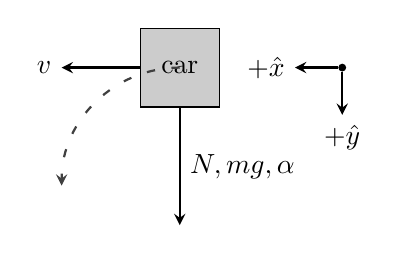
\begin{tikzpicture}
				\node [rectangle, draw = black, fill = black!20, minimum size = 1cm] (origin) { car };
				\draw [thick, -stealth] (origin.west) -- (-1.5cm, 0) node [left] {$ v $};
				\draw [thick, -stealth] (origin.south) -- (0, -2cm) node [midway, right] {$ N, mg, \alpha $};
				\draw [thick, -stealth, black!75, loosely dashed] (origin.center) arc(90:180:1.5cm);

				\node [circle, fill, inner sep = 1pt, right = 1.5cm of origin] (axis_point) {};
				\draw [thick, -stealth] (axis_point) -- ++ (0, -0.6cm) node [below] {$ +\hat{y} $};
				\draw [thick, -stealth] (axis_point) -- ++ (-0.6cm, 0) node [left] {$ +\hat{x} $};
			\end{tikzpicture}
		\end{center}
		\begin{align*}
			\sum F_c & = m\alpha \\
			N + mg & = m \left( \frac{ v^2 }{ r } \right) \\
			N & = m \left( \frac{ v^2 }{ r } \right) - mg \\
			N & = \SI{1.60}{\kilogram} \left( \frac{ (\SI{12.0}{\meter \per \second})^2 }{ \SI{5.00}{\meter} } - \SI{10.0}{\meter \per \second \squared} \right) \\
			N & = \SI{30.1}{\meter \per \second \squared}
		\end{align*}
		\bc{ N = \SI{30.1}{\meter \per \second \squared} }
\end{enumerate}

\subsection{5.48}

\begin{align*}
	r & = \SI{230.0}{\meter} \\
	v & = \SI{28.0}{\meter \per \second}
\end{align*}
\begin{enumerate}[label = \textbf{(\alph*)}]
	\item \label{5.48_a} What is the minimum coefficient of static friction that will prevent sliding?
		\begin{center}
			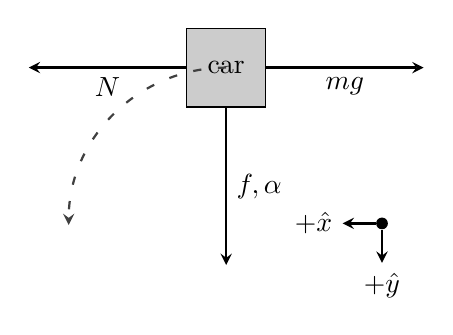
\begin{tikzpicture}
				\node [rectangle, draw = black, fill = black!20, minimum size = 1cm] (car) { car };
				\draw [thick, -stealth] (car.south) -- ++ (0, -2cm) node [midway, right] {$ f, \alpha $};
				\draw [thick, -stealth] (car.west) -- ++ (-2cm, 0) node [midway, below] {$ N $};
				\draw [thick, -stealth] (car.east) -- ++ (2cm, 0) node [midway, below] {$ mg $};
				\draw [thick, -stealth, black!75, loosely dashed] (car.center) arc(90:180:2cm);

				\node [below right = 2cm of car, circle, fill, inner sep = 1.5pt] (axis_point) {};
				\draw [thick, -stealth] (axis_point) -- ++ (-0.5cm, 0) node [left] {$ +\hat{x} $};
				\draw [thick, -stealth] (axis_point) -- ++ (0, -0.5cm) node [below] {$ +\hat{y} $};
			\end{tikzpicture}
		\end{center}
		\begin{align*}
			\sum F_x & = 0 \\
			N & = mg
		\end{align*}
		\begin{align*}
			\sum F_y & = m\alpha \\
			f & = m \left( \frac{ v^2 }{ r } \right) \\
			\mu N & = m \left( \frac{ v^2 }{ r } \right), \quad N = mg \\
			\mu & = \frac{ v^2 }{ rg } \\
			\mu & = \frac{ (\SI{28.0}{\meter \per \second})^2 }{ (\SI{230.0}{\meter})(\SI{10.0}{\meter \per \second \squared}) } \\
			\mu & = 0.341
		\end{align*}
		\bc{ \mu = 0.341 }
	\item Suppose that the highway is icy and the coefficient of static friction between the tires and pavement is only one-third of what you found in part \ref{5.48_a}. What should be the maximum speed of the car so that it can round the curve safely?
		\begin{align*}
			\sum F_y & = m\alpha \\
			\frac{ \mu }{ 3 }mg & = m \left( \frac{ v^2 }{ r } \right) \\
			v & = \sqrt{ \frac{ \mu gr }{ 3 } } \\
			v & = \sqrt{ \frac{ (0.341)(\SI{10.0}{\meter \per \second \squared})(\SI{230.0}{\meter}) }{ 3 } } \\
			v & = \SI{16.2}{\meter \per \second}
		\end{align*}
		\bc{ v = \SI{16.2}{\meter \per \second} }
\end{enumerate}

\subsection{5.54}

\begin{align*}
	D & = \SI{100}{\meter} \\
	r & = \frac{D}{2} = \SI{50.0}{\meter} \\
	\text{rpm} & = \SI{1}{\rev \per \minute}
\end{align*}
\begin{enumerate}[label = \textbf{(\alph*)}]
	\item Find the speed of the passengers when the Ferris wheel is rotating at this rate.
		\begin{align*}
			v & = \frac{ 2\pi r }{ T } \\
			v & = \frac{ 2\pi (\SI{50.0}{\meter}) }{ \SI{60.0}{\second} } \\
			v & = \SI{5.24}{\meter \per \second}
		\end{align*}
		\bc{ v = \SI{5.24}{\meter \per \second} }
	\item A passenger weighs \SI{902}{\newton} at the weight-guessing booth on the ground. What is his apparent weight at the highest and at the lowest point on the Ferris wheel?
		\begin{align*}
			m & = \frac{w}{g} = \frac{ \SI{902}{\newton} }{ \SI{10.0}{\meter \per \second \squared} } = \SI{90.2}{\kilogram}
		\end{align*}
		\begin{align*}
			\sum F_y^{top} & = m\alpha \\
			mg & = m \left( \frac{ v^2 }{ r } \right) + N_{top} \\
			N_{top} & = m \left( -\frac{ v^2 }{ r } + g \right) \\
			N_{top} & = (\SI{90.2}{\kilogram}) \left( -\frac{ (\SI{5.24}{\meter \per \second})^2 }{ \SI{50.0}{\meter} } + \SI{10.0}{\meter \per \second \squared} \right) \\
			N_{top} & = \SI{852.5}{\newton}
		\end{align*}
		\begin{align*}
			\sum F_y^{bottom} & = m\alpha \\
			N_{bottom} & = m \left( \frac{ v^2 }{ r } \right) + mg \\
			N_{bottom} & = m \left( \frac{ v^2 }{ r } + g \right) \\
			N_{bottom} & = (\SI{90.2}{\kilogram}) \left( \frac{ (\SI{5.24}{\meter \per \second})^2 }{ \SI{50.0}{\meter} } + \SI{10.0}{\meter \per \second \squared} \right) \\
			N_{bottom} & = \SI{951.5}{\newton}
		\end{align*}
		\bc{ N_{top} = \SI{852.5}{\newton}, N_{bottom} = \SI{951.5}{\newton} }
	\item What would be the time for one revolution if the passenger’s apparent weight at the highest point were zero?
		\begin{align*}
			v & = \frac{ 2\pi r}{ T } \\
			T & = \frac{ 2\pi r }{ v }
		\end{align*}
		\begin{align*}
			\sum F_y^{top} & = m\alpha \\
			mg & = m \left( \frac{ v^2 }{ r } \right) + N \\
			v & = \sqrt{ gr - \frac{ N }{ m } }, \quad N = 0 \\
			v & = \sqrt{ gr } \\
			v & = \sqrt{ (\SI{10.0}{\meter \per \second \squared})(\SI{50.0}{\meter}) } \\
			v & = \SI{22.4}{\meter \per \second}
		\end{align*}
		\begin{align*}
			T & = \frac{ 2\pi (\SI{50.0}{\meter}) }{ \SI{22.4}{\meter \per \second} } \\
			T & = \SI{14.0}{\second}
		\end{align*}
		\bc{ T = \SI{14.0}{\second} }
\end{enumerate}

\subsection{5.107}

\begin{align*}
	r & = \SI{0.100}{\meter} \\
	\text{rpm} & = \SI{4.80}{\rev \per \second}
\end{align*}
\begin{center}
	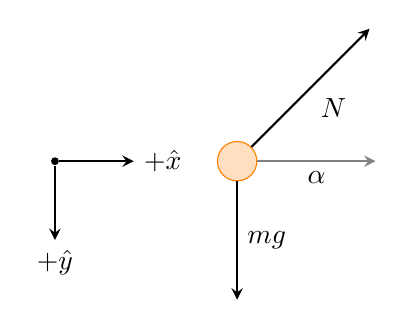
\begin{tikzpicture}
		\node [circle, draw = orange, fill = orange!25, minimum size = 0.5cm] (bead) {};
		\draw [thick, -stealth] (bead.north east) -- ++ (1.5cm, 1.5cm) node [midway, below right] {$ N $};
		\draw [thick, -stealth] (bead.south) -- ++ (0, -1.5cm) node [midway, right] {$ mg $};
		\draw [thick, -stealth, draw = black!50] (bead.east) -- ++ (1.5cm, 0) node [midway, below, black] {$ \alpha $};

		\node [left = 2cm of bead, circle, fill, inner sep = 1pt] (axis_point) {};
		\draw [thick, -stealth] (axis_point) -- ++ (1cm, 0) node [right] {$ +\hat{x} $};
		\draw [thick, -stealth] (axis_point) -- ++ (0, -1cm) node [below] {$ +\hat{y} $};
	\end{tikzpicture}
\end{center}
\begin{enumerate}[label = \textbf{(\alph*)}]
	\item Find the angle $ \beta $ at which the bead is in vertical equilibrium.
		\begin{align*}
			\sum F_x^{bead} & = m\alpha \\
			N_x\sin(\beta) & = m\alpha \\
			N_x & = \frac{ m \frac{ v^2 }{ r } }{ \sin(\beta) } = \frac{ mv^2 }{ r\sin(\beta) }
		\end{align*}
		\begin{align*}
			\sum F_y^{bead} & = 0 \\
			N_y\cos(\beta) & = mg \\
			N_y & = \frac{ mg }{ \cos(\beta) }
		\end{align*}
		\begin{align*}
			N_x & = N_y \\
			\frac{ mv^2 }{ r\sin(\beta) } & = \frac{ mg }{ \cos(\beta) } \\
			v^2\cos(\beta) & = gr\sin(\beta) \\
			\tan(\beta) & = \frac{ v^2 }{ gr } \\
			\beta & = \arctan \left( \frac{ v^2 }{ gr } \right) \\
			\beta & = \arctan \left( \frac{ \left( \frac{ 2\pi r }{ T } \right)^2 }{ gr } \right) \\
			\beta & = \arctan \left( \frac{ 4\pi^2r }{ gT^2 } \right) \\
			\beta & = \arctan \left( \frac{ 4\pi^2(\SI{0.100}{\meter}) }{ (\SI{10.0}{\meter \per \second \squared}) \left( \frac{1}{4.80}\text{s} \right)^2 } \right) \\
			\beta & = \SI{83.7}{\degree}
		\end{align*}
		\bc{ \beta = \SI{83.7}{\degree} }
	\item Is it possible for the bead to ``ride" at the same elevation as the center of the hoop?
		\begin{equation*} \beta = \SI{90.0}{\degree} \end{equation*}
		\begin{align*}
			\frac{ v^2 }{ r\sin(\beta) } & = \frac{ g }{ \cos(\beta) } \\
			v & = \sqrt{ \frac{ gr\sin(\beta) }{ \cos(\beta) } } \\
			v & = \sqrt{ \frac{ (\SI{10.0}{\meter \per \second \squared})(\SI{0.100}{\meter})\sin(\SI{90.0}{\degree}) }{ \cos(\SI{90.0}{\degree}) } } \\
			v & = 0
		\end{align*}
		\begin{mdframed}
			No it is not possible as the velocity would have to be zero, but would instead mean that the bead isn't moving.
		\end{mdframed}
	\item What will happen if the hoop rotates at \SI{1.00}{\rev \per \second}?
		\begin{align*}
			\beta & = \arctan \left( \frac{ 4\pi^2(\SI{0.100}{\meter}) }{ (\SI{10.0}{\meter \per \second \squared})(\SI{1.00}{\second})^2 } \right) \\
			\beta & = \SI{21.5}{\degree}
		\end{align*}
		\begin{mdframed}
			The bead ends up swinging at an angle lower and closer to the vertical axis.
		\end{mdframed}
\end{enumerate}

\section{Lab Manual}

\subsection{1072}

\begin{center}
	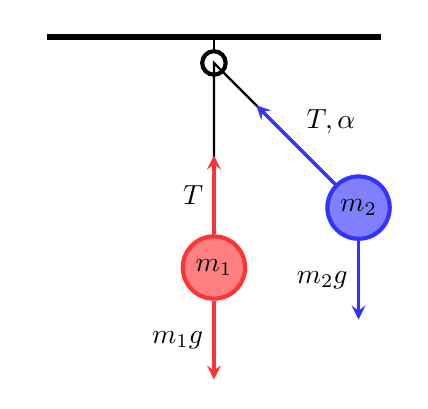
\begin{tikzpicture}
		\node at (0, 0) (origin) {};
		\node [left = 2cm of origin] (left_roof) {};
		\node [right = 2cm of origin] (right_roof) {};

		\draw [line width = 2pt, black] (left_roof) -- (right_roof);

		\draw [thick, black] (origin.center) -- ++ (0, -0.2cm) node (swivel_line) {};

		\node [circle, draw = black, thick, inner sep = 3pt, line width = 1.5pt] at (swivel_line.south) (swivel) {};

		\node [circle, draw = red!80, fill = red!50, inner sep = 3pt, below = 2cm of swivel, line width = 1.5pt] (m_1) {$ m_1 $};
		\node [circle, draw = blue!80, fill = blue!50, inner sep = 3pt, below right = 2cm of swivel, line width = 1.5pt] (m_2) {$ m_2 $};

		\draw [thick, black] (m_1.north) -- (swivel.center) -- (m_2.north west);

		\draw [very thick, draw = red!80, -stealth] (m_1.north) -- ++ (0, 1cm) node [midway, left] {$ T $};
		\draw [very thick, draw = red!80, -stealth] (m_1.south) -- ++ (0, -1cm) node [midway, left] {$ m_1g $};

		\draw [very thick, draw = blue!80, -stealth] (m_2.north west) -- ++ (-1cm, 1cm) node [midway, above right] {$ T, \alpha $};
		\draw [very thick, draw = blue!80, -stealth] (m_2.south) -- ++ (0, -1cm) node [midway, left] {$ m_2g $};
	\end{tikzpicture}
\end{center}
\begin{align*}
	\sum F_y^{m_1} & = 0 \\
	T & = m_1g
\end{align*}
\begin{align*}
	\sum F_y^{m_2} & = m_2g \\
	T\cos(\theta) & = m_2g
\end{align*}
\begin{align*}
	\sum F_x^{m_2} & = m_2\alpha \\
	T\sin(\theta) & = m_2 \left( \frac{ \left( \frac{ 2\pi (c - a) }{ t } \right)^2 }{ c - a } \right) \\
	m_1g\sin(\theta) & = m_2 \left( \frac{ 4\pi^2(c - a) }{ t^2 } \right) \\
	t & = 2\pi \sqrt{ \frac{ m_2(c - a) }{ m_1g } }
\end{align*}
\bc{ t = 2\pi \sqrt{ \frac{ m_2(c - a) }{ m_1g } } }

\subsection{1073}

\begin{align*}
	\sum F_c & = dm\alpha \\
	\sum F_c & = dm\omega^2r
\end{align*}
\begin{align*}
	\sum F_x & = 0 \\
	T\cos \left( \frac{ d\theta }{ 2 } \right) - T \cos \left( \frac{ d\theta }{ 2 } \right) & = 0 \\
	0 & = 0
\end{align*}
\begin{align*}
	\sum F_y & = 0 \\
	2T\sin \left( \frac{ d\theta }{ 2 } \right) & = 0 \\
	Td\theta & = 0
\end{align*}
\begin{align*}
	\sum F_c & = dm\omega^2r \\
	0 + Td\theta & = dm\omega^2r \\
	T & = \frac{dm}{d\theta}\omega^2r \\
	T & = (\rho A r)\omega^2r \\
	T & = \rho A\omega^2r^2
\end{align*}
\bc{ T = \rho A\omega^2R^2 }

\subsection{1082}

\begin{align*}
	v & = \SI{12}{\feet \per \second} \\
	\theta & = \SI{53}{\degree} \\
	m & = \SI{180}{\pound}
\end{align*}
\begin{enumerate}[label = \textbf{(\alph*)}]
	\item Draw a diagram showing all the forces on the bicycle and rider. What direction does he tend to tip (clockwise or counter-clockwise) if he inclines at angle greater than \SI{53}{\degree}? What causes him to tip?
		\begin{center}
			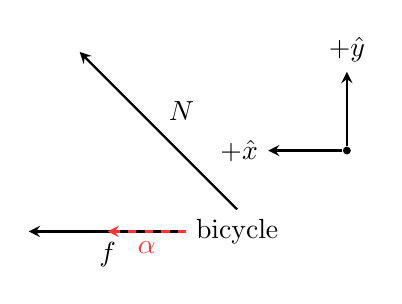
\begin{tikzpicture}
				\node at (0, 0) (bicycle) { bicycle };

				\draw [-stealth, draw = black, thick] (bicycle.west) -- ++ (-2cm, 0) node [midway, below] {$ f $};

				\draw [-stealth, draw = red!80, thick, dashed] (bicycle.west) -- ++ (-1cm, 0) node [midway, below, red!80] {$ \alpha $};

				\draw [-stealth, draw = black, thick] (bicycle.north) -- ++ (-2cm, 2cm) node [midway, above right] {$ N $};

				\node [above right = 1cm of bicycle, circle, fill, inner sep = 1pt] (axis) {};
				\draw [-stealth, draw = black, thick] (axis) -- ++ (-1cm, 0) node [left] {$ +\hat{x} $};
				\draw [-stealth, draw = black, thick] (axis) -- ++ (0, 1cm) node [above] {$ +\hat{y} $};
			\end{tikzpicture}
			\hspace{2cm}
			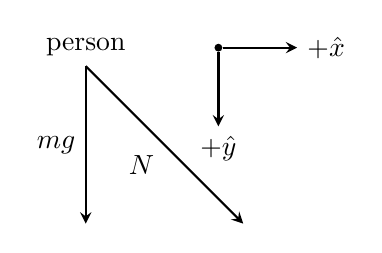
\begin{tikzpicture}
				\node at (0, 0) (person) { person };

				\draw [-stealth, draw = black, thick] (person.south) -- ++ (0, -2cm) node [midway, left] {$ mg $};

				\draw [-stealth, draw = black, thick] (person.south) -- ++ (2cm, -2cm) node [midway, below left] {$ N $};

				\node [right = 1cm of person, circle, fill, inner sep = 1pt] (axis) {};
				\draw [-stealth, draw = black, thick] (axis) -- ++ (1cm, 0) node [right] {$ +\hat{x} $};
				\draw [-stealth, draw = black, thick] (axis) -- ++ (0, -1cm) node [below] {$ +\hat{y} $};
			\end{tikzpicture}
		\end{center}
		\begin{mdframed}
			If he continues to inline at an angle greater than \SI{53}{\degree}, he will begin to tip clockwise. His centripetal force becomes stronger than his weight pulling him down, causing him to tip. A more general answer as to why he tips is if the boy is unable to balance his centripetal force with his (the boy and bicycle's) weight, he will not be able to keep his balance.
		\end{mdframed}
	\item Find the radius of the curve.
		\begin{align*}
			\sum F_y^{(person)} & = 0 \\
			N\sin(\theta) + mg & = 0 \\
			N & = -\frac{ mg }{ \sin(\theta) }
		\end{align*}
		\begin{align*}
			\sum F_x^{(bicycle)} & = m\alpha \\
			N\cos(\theta) & = m\alpha \\
			\left( -\frac{ mg }{ \sin(\theta) } \right) \cos(\theta) & = m \left( \frac{ v^2 }{ r } \right) \\
			-\frac{ gm }{ \tan(\theta) } & = \frac{ mv^2 }{ r } \\
			r & = -\frac{ \tan(\theta)v^2 }{ g } \\
			r & = -\frac{ \tan(\SI{53}{\degree})(\SI{12}{\feet \per \second})^2 }{ \SI{32.17}{\feet \per \second \squared} } \\
			r & = \SI{-5.94}{\meter}
		\end{align*}
		\begin{mdframed}
			The radius is \SI{5.94}{\meter} to the left.
		\end{mdframed}
	\item Find the friction force between the road and wheel.
		\begin{align*}
			\sum F & = 0 \\
			N\cos(\theta) + f & = 0 \\
			f & = -N\cos(\theta) \\
			f & = \frac{ gw }{ \tan(\theta) } \\
			f & = \frac{ \SI{180}{\pound} }{ \tan(\SI{53}{\degree}) } \\
			f & = \SI{136.0}{\pound}
		\end{align*}
		\bc{ f = \SI{136.0}{\pound} }
\end{enumerate}

\subsection{1087}

\begin{center}
	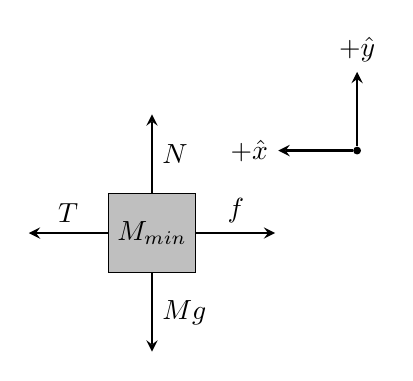
\begin{tikzpicture}
		\node at (0, 0) (origin) {};

		\node [rectangle, draw = black, fill = black!25, minimum size = 1cm] at (origin.center) (M) {$ M_{min} $};
		\draw [-stealth, draw = black, thick] (M.west) -- ++ (-1cm, 0) node [midway, above] {$ T $};
		\draw [-stealth, draw = black, thick] (M.south) -- ++ (0, -1cm) node [midway, right] {$ Mg $};
		\draw [-stealth, draw = black, thick] (M.north) -- ++ (0, 1cm) node [midway, right] {$ N $};
		\draw [-stealth, draw = black, thick] (M.east) -- ++ (1cm, 0) node [midway, above] {$ f $};

		\node [above right = 0.5cm and 2cm of M, circle, fill, inner sep = 1pt] (axis) {};
		\draw [-stealth, draw = black, thick] (axis) -- ++ (-1cm, 0) node [left] {$ +\hat{x} $};
		\draw [-stealth, draw = black, thick] (axis) -- ++ (0, 1cm) node [above] {$ +\hat{y} $};
	\end{tikzpicture}
	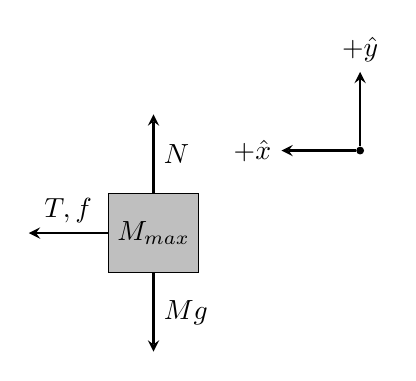
\begin{tikzpicture}
		\node at (0, 0) (origin) {};

		\node [rectangle, draw = black, fill = black!25, minimum size = 1cm] at (origin.center) (M) {$ M_{max} $};
		\draw [-stealth, draw = black, thick] (M.west) -- ++ (-1cm, 0) node [midway, above] {$ T, f $};
		\draw [-stealth, draw = black, thick] (M.south) -- ++ (0, -1cm) node [midway, right] {$ Mg $};
		\draw [-stealth, draw = black, thick] (M.north) -- ++ (0, 1cm) node [midway, right] {$ N $};

		\node [above right = 0.5cm and 2cm of M, circle, fill, inner sep = 1pt] (axis) {};
		\draw [-stealth, draw = black, thick] (axis) -- ++ (-1cm, 0) node [left] {$ +\hat{x} $};
		\draw [-stealth, draw = black, thick] (axis) -- ++ (0, 1cm) node [above] {$ +\hat{y} $};
	\end{tikzpicture}
	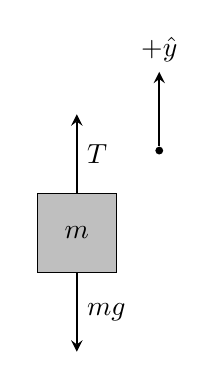
\begin{tikzpicture}
		\node at (0, 0) (origin) {};

		\node [rectangle, draw = black, fill = black!25, minimum size = 1cm] at (origin.center) (m) {$ m $};

		\draw [-stealth, draw = black, thick] (m.north) -- ++ (0, 1cm) node [midway, right] {$ T $};
		\draw [-stealth, draw = black, thick] (m.south) -- ++ (0, -1cm) node [midway, right] {$ mg $};

		\node [below = 0.25cm of m.south west] (acceleration) {};

		\node [above right = 0.5cm and 0.5cm of m, circle, fill, inner sep = 1pt] (axis) {};
		\draw [-stealth, draw = black, thick] (axis) -- ++ (0, 1cm) node [above] {$ +\hat{y} $};
	\end{tikzpicture}
\end{center}
\begin{align*}
	\sum F_y^{(m)} & = 0 \\
	T & = mg
\end{align*}
\begin{align*}
	\sum F_y^{(M)} & = 0 \\
	N & = Mg
\end{align*}
\begin{align*}
	\sum F_x^{(M)} & = M\omega^2\mu_{min} \\
	T & = M\omega^2\mu_{min} + f \\
	\mu_{min} & = \frac{ T - f }{ M\omega^2 } \\
	\mu_{min} & = \frac{ mg - \mu Mg }{ M\omega^2 }
\end{align*}
\begin{align*}
	\sum F_x^{(M)} & = M\omega^2\mu_{max} \\
	T + f & = M\omega^2\mu_{max} \\
	\mu_{max} & = \frac{ T + f }{ M\omega^2 } \\
	\mu_{max} & = \frac{ mg + \mu Mg }{ M\omega^2 }
\end{align*}
\bc {
	\mu_{min} = \frac{ mg - \mu Mg }{ M\omega^2 }, \mu_{max} = \frac{ mg + \mu Mg }{ M\omega^2 }
}

\subsection{1088}

\begin{align*}
	\sum F_x & = m\alpha \\
	N\sin(\theta) & = m \left( \frac{ v^2 }{ L\cos(\theta) } \right)
\end{align*}
\begin{align*}
	\sum F_y & = 0 \\
	N\cos(\theta) & = mg
\end{align*}
\begin{align*}
	\frac{ N\sin(\theta) }{ N \cos(\theta) } & = \frac{ m \left( \frac{ v^2 }{ L\cos(\theta) } \right) }{ mg } \\
	\tan(\theta) & = \frac{ v^2 }{ gL\cos(\theta) } \\
	v & = \sqrt{ gL\sin(\theta) }
\end{align*}
\bc{ v = \sqrt{ gL\sin(\theta) } }

\begin{align*}
	m\lap[\ddot{x}] + b\lap[\dot{x}] + k\lap[x] & = \lap[0] \\
	m \left[ s^2\lap[x] - sx(0) - \dot{x}(0) \right] + b \left[ s\lap[x] - x(0) \right] + k\lap[x] & = 0 \\
	\lap[x](ms^2 + bs + k) - smx(0) - m\dot{x}(0) - bx(0) & = 0 \\
	\lap[x] & = \frac{ smx(0) + m\dot{x}(0) + bx(0) }{ ms^2 + bs + k } \\
	x & = \ilap[ \frac{ smx(0) + m\dot{x}(0) + bx(0) }{ ms^2 + bs + k } ]
\end{align*}

\end{document}
